\documentclass{standalone}
\usepackage{tikz}
\usetikzlibrary{patterns, positioning}

\begin{document}
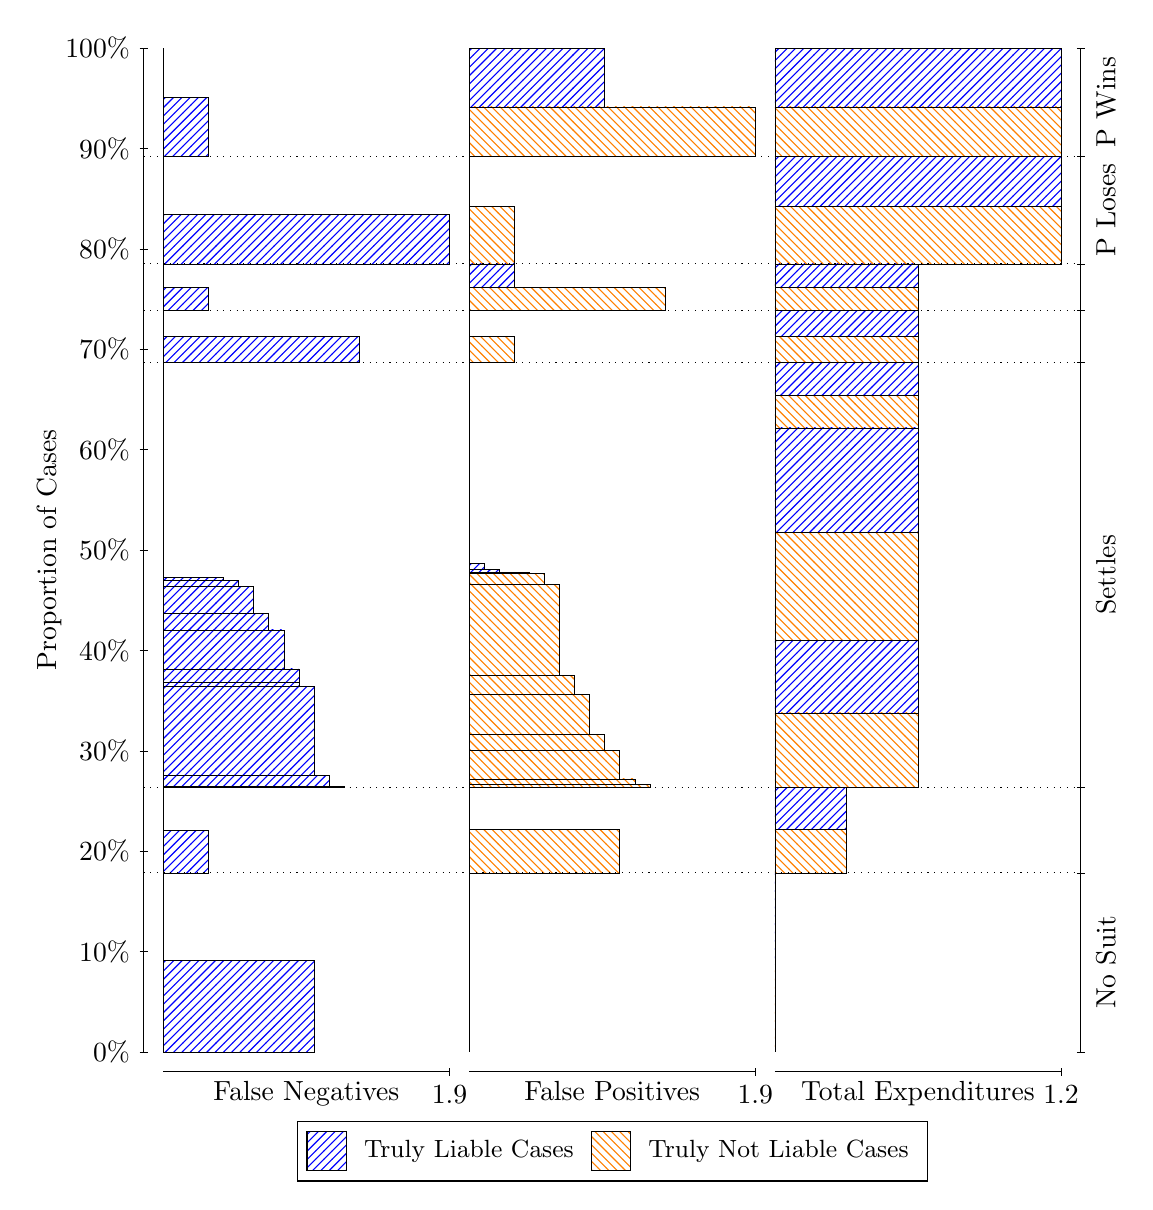
\begin{tikzpicture}
\draw[black, very thin] (1.5,1.75) -- (1.5,14.5);
\node[rotate=90, anchor=center] at (0.3, 8.125) {Proportion of Cases};
\draw[black, very thin] (1.45,1.75) -- (1.55,1.75);
\node[anchor=east] at (1.45, 1.75) {0\%};
\draw[black, very thin] (1.45,3.025) -- (1.55,3.025);
\node[anchor=east] at (1.45, 3.025) {10\%};
\draw[black, very thin] (1.45,4.3) -- (1.55,4.3);
\node[anchor=east] at (1.45, 4.3) {20\%};
\draw[black, very thin] (1.45,5.575) -- (1.55,5.575);
\node[anchor=east] at (1.45, 5.575) {30\%};
\draw[black, very thin] (1.45,6.85) -- (1.55,6.85);
\node[anchor=east] at (1.45, 6.85) {40\%};
\draw[black, very thin] (1.45,8.125) -- (1.55,8.125);
\node[anchor=east] at (1.45, 8.125) {50\%};
\draw[black, very thin] (1.45,9.4) -- (1.55,9.4);
\node[anchor=east] at (1.45, 9.4) {60\%};
\draw[black, very thin] (1.45,10.675) -- (1.55,10.675);
\node[anchor=east] at (1.45, 10.675) {70\%};
\draw[black, very thin] (1.45,11.95) -- (1.55,11.95);
\node[anchor=east] at (1.45, 11.95) {80\%};
\draw[black, very thin] (1.45,13.225) -- (1.55,13.225);
\node[anchor=east] at (1.45, 13.225) {90\%};
\draw[black, very thin] (1.45,14.5) -- (1.55,14.5);
\node[anchor=east] at (1.45, 14.5) {100\%};

\draw[black, very thin] (13.4,1.75) -- (13.4,14.5);
\draw[black, very thin] (13.35,1.75) -- (13.45,1.75);
\node[anchor=west] at (13.35, 1.75) {};
\draw[black, very thin] (13.35,4.0237) -- (13.45,4.0237);
\node[anchor=west] at (13.35, 4.0237) {};
\draw[black, very thin] (13.35,5.114) -- (13.45,5.114);
\node[anchor=west] at (13.35, 5.114) {};
\draw[black, very thin] (13.35,10.505) -- (13.45,10.505);
\node[anchor=west] at (13.35, 10.505) {};
\draw[black, very thin] (13.35,11.168) -- (13.45,11.168);
\node[anchor=west] at (13.35, 11.168) {};
\draw[black, very thin] (13.35,11.758) -- (13.45,11.758);
\node[anchor=west] at (13.35, 11.758) {};
\draw[black, very thin] (13.35,13.127) -- (13.45,13.127);
\node[anchor=west] at (13.35, 13.127) {};
\draw[black, very thin] (13.35,14.5) -- (13.45,14.5);
\node[anchor=west] at (13.35, 14.5) {};

\draw[black, very thin, pattern color=blue, pattern=north east lines] (1.75,1.75) rectangle (3.6623,2.9172);
\draw[black, very thin, pattern color=orange, pattern=north west lines] (1.75,2.9172) rectangle (1.75,4.0237);
\draw[black, very thin, pattern color=blue, pattern=north east lines] (1.75,4.0237) rectangle (2.3237,4.5619);
\draw[black, very thin, pattern color=orange, pattern=north west lines] (1.75,4.5619) rectangle (1.75,5.114);
\draw[black, very thin, pattern color=blue, pattern=north east lines] (1.75,5.114) rectangle (4.0447,5.1264);
\draw[black, very thin, pattern color=blue, pattern=north east lines] (1.75,5.1264) rectangle (3.8535,5.2625);
\draw[black, very thin, pattern color=blue, pattern=north east lines] (1.75,5.2625) rectangle (3.6623,6.389);
\draw[black, very thin, pattern color=blue, pattern=north east lines] (1.75,6.389) rectangle (3.4711,6.4431);
\draw[black, very thin, pattern color=blue, pattern=north east lines] (1.75,6.4431) rectangle (3.4711,6.6163);
\draw[black, very thin, pattern color=blue, pattern=north east lines] (1.75,6.6163) rectangle (3.2798,7.1102);
\draw[black, very thin, pattern color=blue, pattern=north east lines] (1.75,7.1102) rectangle (3.0886,7.3175);
\draw[black, very thin, pattern color=blue, pattern=north east lines] (1.75,7.3175) rectangle (2.8974,7.6678);
\draw[black, very thin, pattern color=blue, pattern=north east lines] (1.75,7.6678) rectangle (2.7061,7.7419);
\draw[black, very thin, pattern color=blue, pattern=north east lines] (1.75,7.7419) rectangle (2.5149,7.7743);
\draw[black, very thin, pattern color=orange, pattern=north west lines] (1.75,7.7743) rectangle (1.75,10.505);
\draw[black, very thin, pattern color=blue, pattern=north east lines] (1.75,10.505) rectangle (4.236,10.838);
\draw[black, very thin, pattern color=orange, pattern=north west lines] (1.75,10.838) rectangle (1.75,11.168);
\draw[black, very thin, pattern color=blue, pattern=north east lines] (1.75,11.168) rectangle (2.3237,11.463);
\draw[black, very thin, pattern color=orange, pattern=north west lines] (1.75,11.463) rectangle (1.75,11.758);
\draw[black, very thin, pattern color=blue, pattern=north east lines] (1.75,11.758) rectangle (5.3833,12.392);
\draw[black, very thin, pattern color=orange, pattern=north west lines] (1.75,12.392) rectangle (1.75,13.127);
\draw[black, very thin, pattern color=blue, pattern=north east lines] (1.75,13.127) rectangle (2.3237,13.874);
\draw[black, very thin, pattern color=orange, pattern=north west lines] (1.75,13.874) rectangle (1.75,14.5);
\draw[black, very thin, pattern color=orange, pattern=north west lines] (5.6333,1.75) rectangle (5.6333,2.8564);
\draw[black, very thin, pattern color=blue, pattern=north east lines] (5.6333,2.8564) rectangle (5.6333,4.0237);
\draw[black, very thin, pattern color=orange, pattern=north west lines] (5.6333,4.0237) rectangle (7.5456,4.5758);
\draw[black, very thin, pattern color=blue, pattern=north east lines] (5.6333,4.5758) rectangle (5.6333,5.114);
\draw[black, very thin, pattern color=orange, pattern=north west lines] (5.6333,5.114) rectangle (7.9281,5.1439);
\draw[black, very thin, pattern color=orange, pattern=north west lines] (5.6333,5.1439) rectangle (7.7368,5.2177);
\draw[black, very thin, pattern color=orange, pattern=north west lines] (5.6333,5.2177) rectangle (7.5456,5.5754);
\draw[black, very thin, pattern color=orange, pattern=north west lines] (5.6333,5.5754) rectangle (7.3544,5.7842);
\draw[black, very thin, pattern color=orange, pattern=north west lines] (5.6333,5.7842) rectangle (7.1632,6.2956);
\draw[black, very thin, pattern color=orange, pattern=north west lines] (5.6333,6.2956) rectangle (6.9719,6.5292);
\draw[black, very thin, pattern color=orange, pattern=north west lines] (5.6333,6.5292) rectangle (6.7807,7.6915);
\draw[black, very thin, pattern color=orange, pattern=north west lines] (5.6333,7.6915) rectangle (6.5895,7.8324);
\draw[black, very thin, pattern color=orange, pattern=north west lines] (5.6333,7.8324) rectangle (6.3982,7.8449);
\draw[black, very thin, pattern color=blue, pattern=north east lines] (5.6333,7.8449) rectangle (6.0158,7.8774);
\draw[black, very thin, pattern color=blue, pattern=north east lines] (5.6333,7.8774) rectangle (5.8246,7.9514);
\draw[black, very thin, pattern color=blue, pattern=north east lines] (5.6333,7.9514) rectangle (5.6333,10.505);
\draw[black, very thin, pattern color=orange, pattern=north west lines] (5.6333,10.505) rectangle (6.207,10.834);
\draw[black, very thin, pattern color=blue, pattern=north east lines] (5.6333,10.834) rectangle (5.6333,11.168);
\draw[black, very thin, pattern color=orange, pattern=north west lines] (5.6333,11.168) rectangle (8.1193,11.463);
\draw[black, very thin, pattern color=blue, pattern=north east lines] (5.6333,11.463) rectangle (6.207,11.758);
\draw[black, very thin, pattern color=orange, pattern=north west lines] (5.6333,11.758) rectangle (6.207,12.493);
\draw[black, very thin, pattern color=blue, pattern=north east lines] (5.6333,12.493) rectangle (5.6333,13.127);
\draw[black, very thin, pattern color=orange, pattern=north west lines] (5.6333,13.127) rectangle (9.2667,13.753);
\draw[black, very thin, pattern color=blue, pattern=north east lines] (5.6333,13.753) rectangle (7.3544,14.5);
\draw[black, very thin, pattern color=orange, pattern=north west lines] (9.5167,1.75) rectangle (9.5167,2.8564);
\draw[black, very thin, pattern color=blue, pattern=north east lines] (9.5167,2.8564) rectangle (9.5167,4.0237);
\draw[black, very thin, pattern color=orange, pattern=north west lines] (9.5167,4.0237) rectangle (10.425,4.5758);
\draw[black, very thin, pattern color=blue, pattern=north east lines] (9.5167,4.5758) rectangle (10.425,5.114);
\draw[black, very thin, pattern color=orange, pattern=north west lines] (9.5167,5.114) rectangle (11.333,6.0569);
\draw[black, very thin, pattern color=blue, pattern=north east lines] (9.5167,6.0569) rectangle (11.333,6.9751);
\draw[black, very thin, pattern color=orange, pattern=north west lines] (9.5167,6.9751) rectangle (11.333,8.3473);
\draw[black, very thin, pattern color=blue, pattern=north east lines] (9.5167,8.3473) rectangle (11.333,9.6764);
\draw[black, very thin, pattern color=orange, pattern=north west lines] (9.5167,9.6764) rectangle (11.333,10.092);
\draw[black, very thin, pattern color=blue, pattern=north east lines] (9.5167,10.092) rectangle (11.333,10.505);
\draw[black, very thin, pattern color=orange, pattern=north west lines] (9.5167,10.505) rectangle (11.333,10.834);
\draw[black, very thin, pattern color=blue, pattern=north east lines] (9.5167,10.834) rectangle (11.333,11.168);
\draw[black, very thin, pattern color=orange, pattern=north west lines] (9.5167,11.168) rectangle (11.333,11.463);
\draw[black, very thin, pattern color=blue, pattern=north east lines] (9.5167,11.463) rectangle (11.333,11.758);
\draw[black, very thin, pattern color=orange, pattern=north west lines] (9.5167,11.758) rectangle (13.15,12.493);
\draw[black, very thin, pattern color=blue, pattern=north east lines] (9.5167,12.493) rectangle (13.15,13.127);
\draw[black, very thin, pattern color=orange, pattern=north west lines] (9.5167,13.127) rectangle (13.15,13.753);
\draw[black, very thin, pattern color=blue, pattern=north east lines] (9.5167,13.753) rectangle (13.15,14.5);
\draw[black, dotted] (1.5,4.0237) -- (13.4,4.0237);
\draw[black, dotted] (1.5,5.114) -- (13.4,5.114);
\draw[black, dotted] (1.5,10.505) -- (13.4,10.505);
\draw[black, dotted] (1.5,11.168) -- (13.4,11.168);
\draw[black, dotted] (1.5,11.758) -- (13.4,11.758);
\draw[black, dotted] (1.5,13.127) -- (13.4,13.127);
\draw[black, very thin] (1.75,1.5) -- (5.3833,1.5);
\node[anchor=north] at (3.5667, 1.5) {False Negatives};
\draw[black, very thin] (5.3833,1.45) -- (5.3833,1.55);
\node[anchor=north] at (5.3833, 1.45) {1.9};

\draw[black, very thin] (5.6333,1.5) -- (9.2667,1.5);
\node[anchor=north] at (7.45, 1.5) {False Positives};
\draw[black, very thin] (9.2667,1.45) -- (9.2667,1.55);
\node[anchor=north] at (9.2667, 1.45) {1.9};

\draw[black, very thin] (9.5167,1.5) -- (13.15,1.5);
\node[anchor=north] at (11.333, 1.5) {Total Expenditures};
\draw[black, very thin] (13.15,1.45) -- (13.15,1.55);
\node[anchor=north] at (13.15, 1.45) {1.2};

\node[black, centered, rotate=90] at (13.72, 2.8868) {No Suit};

\node[black, centered, rotate=90] at (13.72, 7.8096) {Settles};


\node[black, centered, rotate=90] at (13.72, 12.443) {P Loses};
\node[black, centered, rotate=90] at (13.72, 13.814) {P Wins};

\draw (7.449999999999999,1.5) node[draw=none] (baseCoordinate) {};
\begin{scope}[align=center]
        \matrix[scale=0.5, draw=black, below=0.5cm of baseCoordinate, nodes={draw}, column sep=0.1cm]{
            \node[rectangle, draw, minimum width=0.5cm, minimum height=0.5cm, pattern=north east lines, pattern color=blue] {}; &
            \node[draw=none, font=\small] (B) {Truly Liable Cases}; &
            \node[rectangle, draw, minimum width=0.5cm, minimum height=0.5cm, pattern=north west lines, pattern color=orange] {}; &
            \node[draw=none, font=\small] (B) {Truly Not Liable Cases}; \\
            };
\end{scope}

\end{tikzpicture}
\end{document}